\chapter{Software and Analysis} \label{ch:software}

\section{Neutron Detectors}

Chapter \ref{ch:neutrons} will go into depth about most of the new additions to the neutron analysis, but some processing and basic cuts must be applied to prepare the data.


\subsection{Pulse Interpolation}

The neutron digitizers operate at a frequency of 170 MHz, corresponding to a bin width of 5.88 ns.
For a significant portion of the 2015 production run an alternate version of the digitizer firmware was used which halved the frequency, producing bin widths of 11.76 ns.
The resulting wave-forms are too coarsely binned to accurately capture the shapes of the pulses, which are quite important for distinguishing neutron and gamma pulses.
In order to produce a more useful input, we perform a spline interpolation of the original waveform.

A simple cubic spline was previously used for the pulse interpolation, but had some undesirable effects.  
In particular, the sharp rise at the start of the pulse produces a spurious undershoot and often produces an oscillating waveform as shown in figure \ref{fig:neu_interp}.
A solution to these issues is to use a constrained spline designed for engineering applications \footnote{http://www.korf.co.uk/spline.pdf} which prevents these effects.
The constrained spline explicitly sets the derivatives at each sample point according to the formula:
\begin{equation}
f'(x_i) = \cfrac{2}{\cfrac{x_{i+1}-x_i}{y_{i+1}-y_i}+\cfrac{x_i-x_{i+1}}{y_i-y_{i+1}}}
\end{equation}
The end points and local extrema require different formulas:
\begin{equation}
f'(x_i) = \begin{cases} 
  0                                                                         & \text{at local extrema} \\
  \frac{3(y_1-y_0)}{2(x_1-x_0)}-\frac{(f'(x_1))}{2}                         & i=0                     \\
  \frac{3(y_n-y_{n-1})}{2(x_n-x_{n-1})}-\frac{(f'(x_{n-1}))}{2}             & i=n               
  \end{cases}
\end{equation}

The constrained spline produces more sensible behavior in the area around the peak, but severely distorts the shape at the top of the peak.  
To produce an interpolated waveform with the benefits of both methods, we create a new spline which blends between the two.
For samples below 10\% of the maximum pulse height the spline derivatives are set according to the constrained spline formula, while samples above 20\% of the maximum height are set according to the natural spline.
Samples between 10\% and 20\% of the maximum have their derivatives set to a weighted average of the two splines.
In this way, we produce a final waveform that closely matches the shape of the natural spline near the peak of the pulse, while minimizing excessive undershoots and oscillations.
A comparison of these methods is shown in figure\ref{fig:neu_interp}.

\begin{figure}[h]
  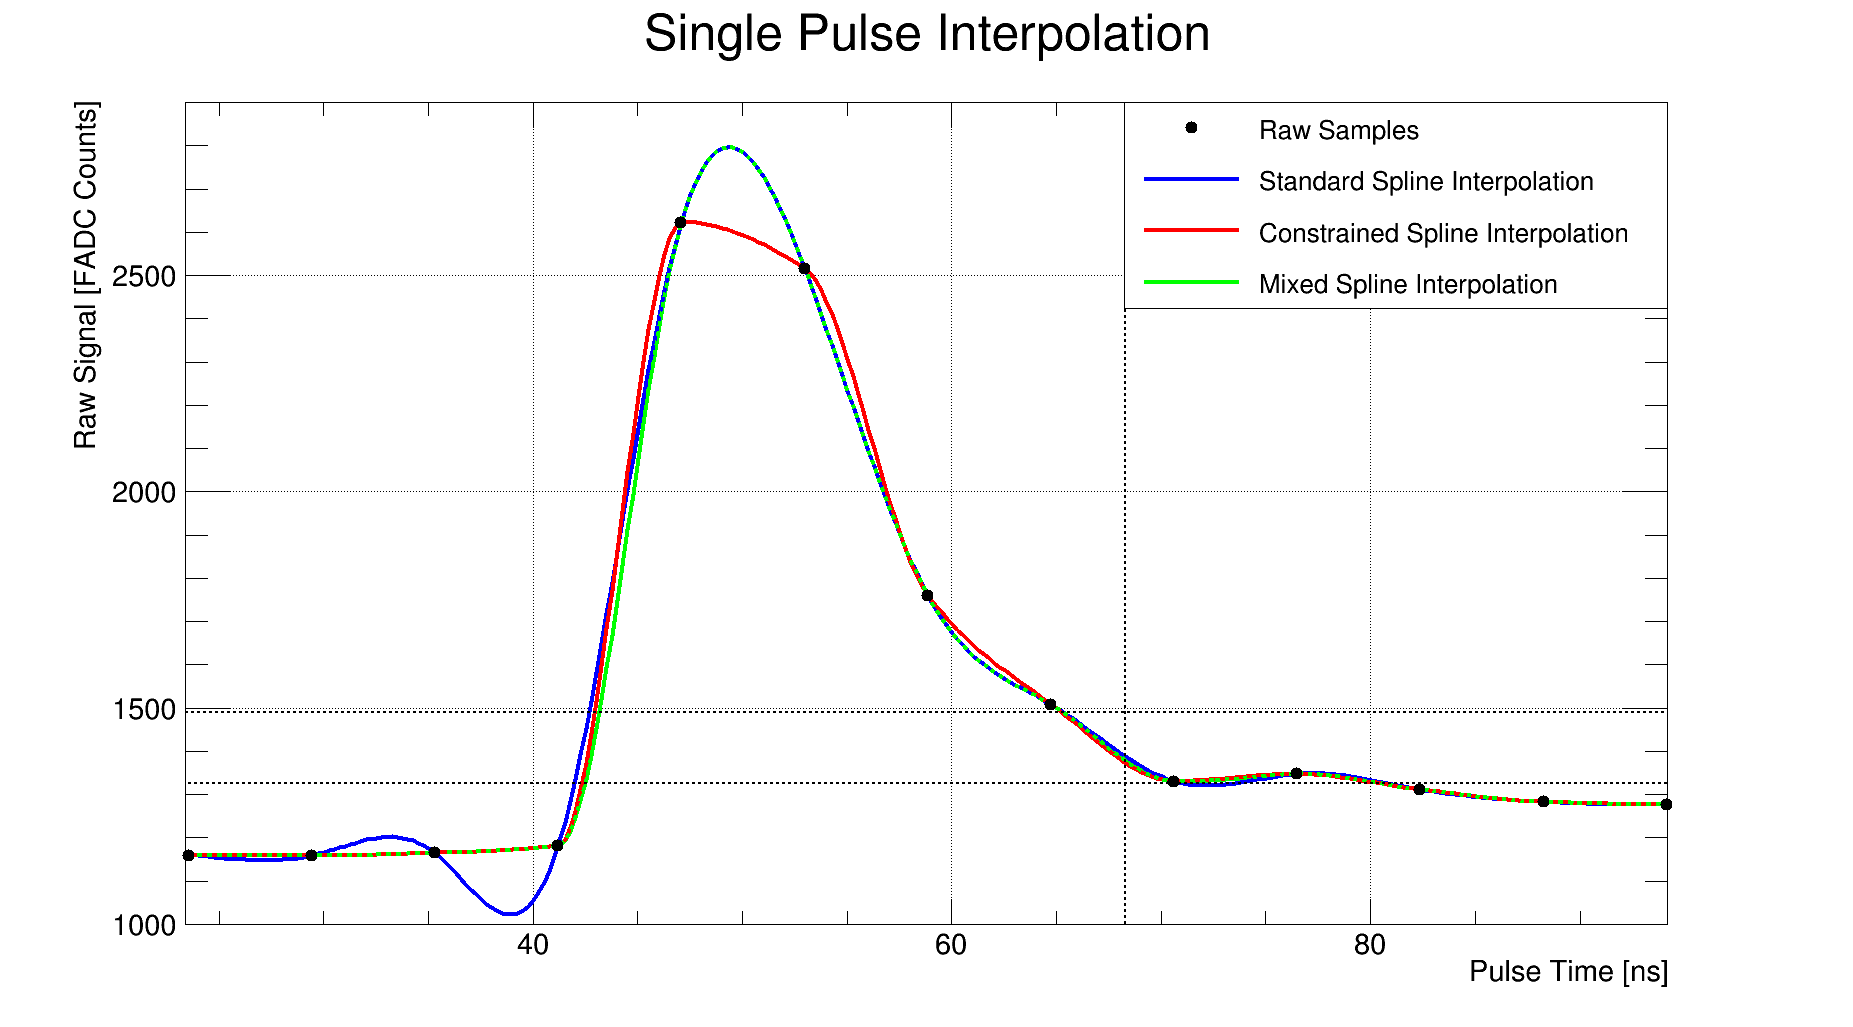
\includegraphics[width=\textwidth]{software/figures/Neutron_Interpolation.png}
  \caption{Interpolated neutron pulse shapes. Black dots indicate raw sample points, the blue curve is a natural spline interpolation, and the red curve is the constrained spline.  The green curve indicates the final combined result. The horizontal dashed lines indicate the 10\%, and 20\% pulse height levels.}
  \label{fig:neu_interp}
\end{figure}

Information about the neutron pulse is then derived from this spline interpolation.
The pulse time is determined by where the rising edge of the pulse passes above 50\% of the maximum height of the spline.
The pulse area is calculated by integrating from $-40 ns$ to $200 ns$ relative to the peak, which should be a window wide enough to capture the entire waveform.
It is assumed that only one pulse exists in a given trace, which is justified given the low rate of neutron events.
A simple check is included to make sure there are no additional large pulses, but a fairly loose threshold is used to avoid false positives.

\subsection{Standard Cuts}

A variety of cuts are made to clean up the neutron data before any real analysis is performed on it.
First standard event cuts are applied such as requiring a 'best entrance' and a clean data block without errors.
In general we also require events to have a lone muon stop detected in the TPC.
Relaxing the TPC stop requirement results in a large number of neutrons associated with muon stops upstream in the beam pipe, which are not particularly relevant for the analysis.
We also separate the muon clock events out for separate analysis.

When it comes to neutron specific cuts, we have in order:
\begin{enumerate}
  \item We require events to have a neutron detector hit between $-20 \mu s$ and $+25 \mu s$ relative to the muon. 
  \item An amplitude threshold is applied for each detector.  Any pulses falling below the threshold will be considered random noise and ignored.
  \item To avoid after-pulsing, events with multiple neutron islands in a given detector are vetoed.  Events where multiple peaks are identified in a given neutron island are also rejected.  However, events with multiple neutrons detected in different detectors are perfectly valid.
  \item Overflow pulses are rejected, and are most likely produced by muons directly entering the neutron detectors and therefore not important for the neutron analysis.
  \item To avoid the possibility of electrons interacting directly in the neutron detectors, events with a prompt coincidence between a neutron pulse and an electron detection may also be vetoed.  This cut causes some complications though, which will be discussed in chapter \ref{ch:neutrons}, and is therefore not always applied.  
  \item Pulse shape discrimination (PSD) cuts are applied to differentiate between neutrons and gamma rays, as detailed in the following section.
\end{enumerate}

\subsection{Pulse Shape Discrimination}

Neutron and gamma ray pulses have distinctive shapes which can be used to identify the event type.
Gamma pulses have a short peak which decays away quickly, while neutron pulses have a more extended tail after the initial peak.
A comparison of averaged waveforms from each event type is shown in figure \ref{fig:neu_tail}.

\begin{figure}[h]
  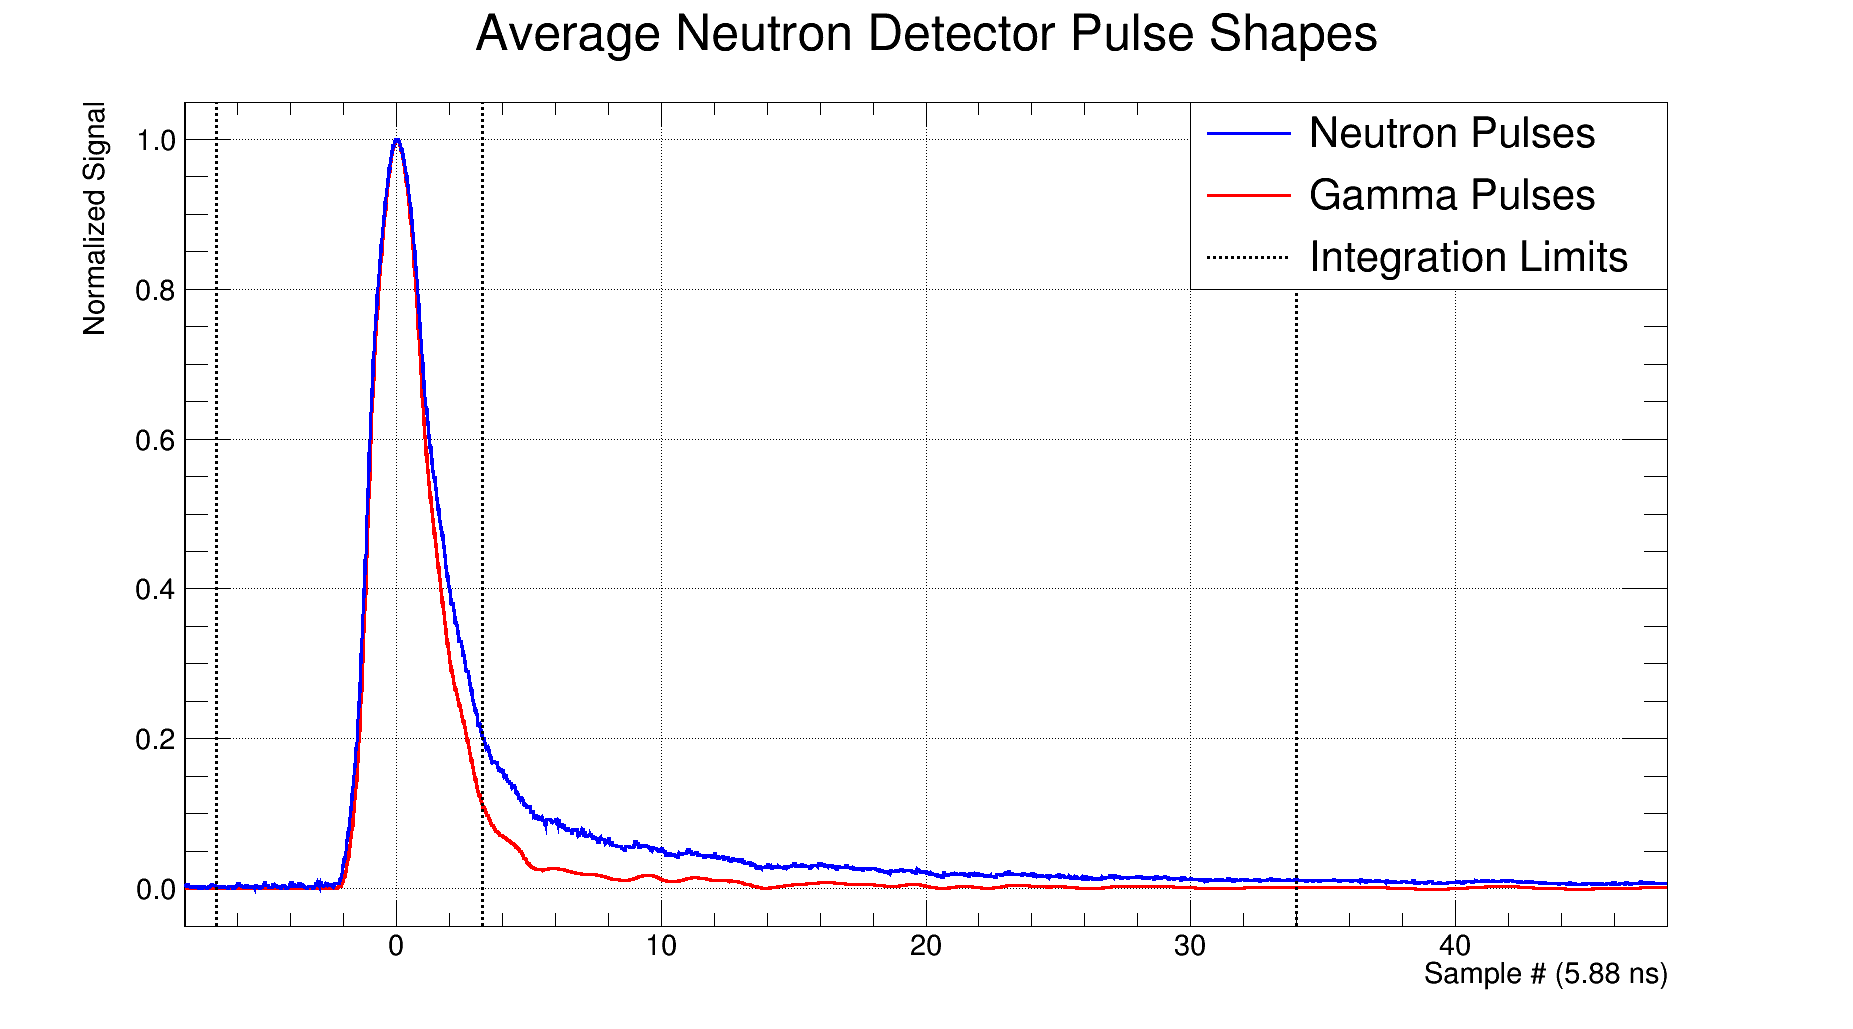
\includegraphics[width=\textwidth]{software/figures/Neutron_Waveform_Averages.png}
  \caption{Comparison of neutron and gamma pulse shapes.  Vertical dashed lines indicate the integration range used for the PSD.}
  \label{fig:neu_tail}
\end{figure}

To quantify the pulse shape, we take the integral in the range from $19 ns$ to $200 ns$ after the peak.
Dividing this tail integral by the total pulse integral gives us the fraction of pulse energy contained in the tail.
We create a two dimensional plot of the tail fraction against the pulse integral, which we refer to as a PSD plot.
An example of a PSD plot is shown in figure \ref{fig:neu_psd}, where we see separate bands produced by the gamma and neutron pulses.
The integration range has been empirically optimized to maximize the separation between these two bands.

\begin{figure}[h]
  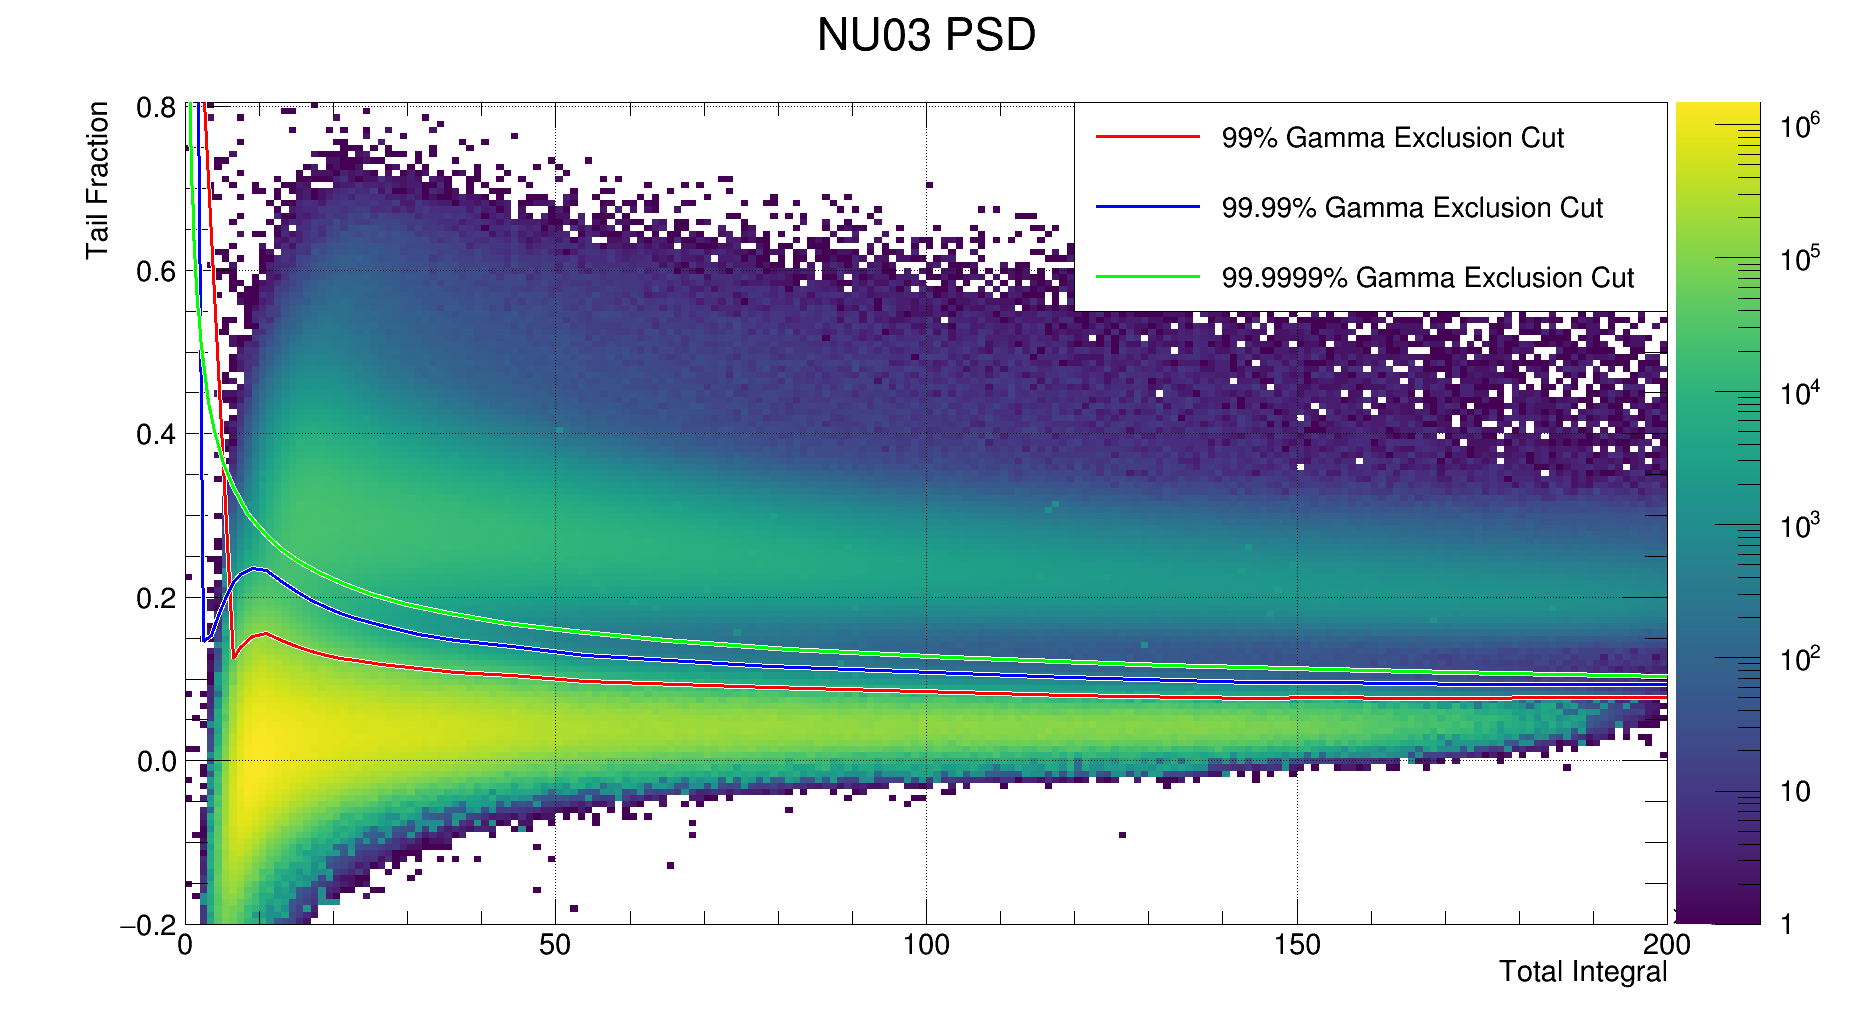
\includegraphics[width=\textwidth]{software/figures/Neutron_PSD.png}
  \caption{Neutron PSD plot for detector NU03.  Three PSD cuts with various levels of strictness are indicated by the colored lines.}
  \label{fig:neu_psd}
\end{figure}

A PSD cut is defined as a curve separating these two bands, with pulses below the curve classified as gamma rays and pulses above the line classified as neutrons.  
Initially PSD cuts were defined by separating the PSD plots into energy slices and fitting each slice with a pair of Gaussian functions.  
The two Gaussians are then assumed to approximately match the distributions of the gamma and neutron events, respectively.
In general there are far more gamma events than neutrons, so the cuts are calculated to exclude a given fraction of the Gaussian fit to the gamma events.
This process produces a cut value for each slice of the PSD plot, which are interpolated linearly to form a continuous curve.
A set of cuts defined with various target exclusion fractions are overlaid on the PSD plot in figure \ref{fig:neu_psd}.
There is little reason to think that the tails of the distributions actually match a Gaussian function, so the stated exclusions are only meaningful relative to each other and should not be taken literally. 

A more sophisticated method of generating PSD cuts has also been developed, relying on comparison of neutron and gamma-selected variants of the PSD plots.
These new cuts have more well defined exclusion fractions and efficiencies.
However, as the creation of these cuts relies on understanding the various neutron and gamma signal sources, a detailed description of them will be left for chapter \ref{ch:neutrons}.